\section{Results}
\label{sec:results}

\subsection{No accuracy tax on pattern matching or factual recall (H1)}
\label{sec:h1}

\Tabref{tab:category} and \figref{fig:delta} give the category-level effect of \CoT.
For pattern matching, $\Delta$ lies between $-1.2$ and $+0.7$ points at every size, and the lower confidence bound is never below $-3.2$, so the main prompt excludes a 5-point tax.
For factual recall, $\Delta$ lies between $-2.2$ and $+3.8$ points.
A 5-point tax is excluded from 1.5B up; at 0.5B the interval $[-5.8, +1.5]$ just reaches it.
None of the ten cells is in the hypothesised range and none is significantly negative.
At 7B and 14B, recall moves slightly in favour of \CoT ($+3.8$ and $+2.8$); the bootstrap intervals exclude zero but neither cell survives Holm correction.
\triviaqa drives this movement (\tabref{tab:task}).

The closest thing to H1 at the task level is the 0.5B model on \mmlu ($-6.0$ points, interval $[-13.0, +1.0]$, not significant).
No task shows a Holm-significant \CoT penalty at any size.

\begin{table}[t]
    \centering
    \caption{\CoT effect $\Delta$ by category and model size, in accuracy points, with 95\% bootstrap intervals. \sig marks Holm-significant cells ($\alpha = 0.05$, 20 tests). The one cell that is both inside its hypothesised range and significant is in {\bf bold}.}
    \label{tab:category}
    \resizebox{\textwidth}{!}{%
    \begin{tabular}{@{}lcccccc@{}}
        \toprule
        \textbf{Category} & \textbf{0.5B} & \textbf{1.5B} & \textbf{3B} & \textbf{7B} & \textbf{14B} & \textbf{Hypothesised} \\
        \midrule
        Pattern matching  & $-0.7$ {\scriptsize $[-3.2, +1.8]$} & $-1.2$ {\scriptsize $[-3.2, +0.8]$} & $+0.7$ {\scriptsize $[-1.2, +2.5]$} & $-0.2$ {\scriptsize $[-1.5, +1.2]$} & $\phantom{+}0.0$ {\scriptsize $[-1.2, +1.2]$} & $-15$ to $-5$ \\
        Factual recall    & $-2.2$ {\scriptsize $[-5.8, +1.5]$} & $-0.2$ {\scriptsize $[-3.5, +3.2]$} & $+1.8$ {\scriptsize $[-1.2, +4.8]$} & $+3.8$ {\scriptsize $[+1.2, +6.5]$} & $+2.8$ {\scriptsize $[+0.3, +5.3]$} & $-15$ to $-5$ \\
        Logical deduction & $-6.9$ {\scriptsize $[-12.3, -1.5]$} & $+7.2$ {\scriptsize $[+2.2, +12.3]$} & $\mathbf{+13.9}$\sig {\scriptsize $[+8.8, +18.8]$} & $+26.7$\sig {\scriptsize $[+21.8, +31.6]$} & $+28.7$\sig {\scriptsize $[+24.2, +33.3]$} & $+10$ to $+25$ \\
        Arithmetic        & $+47.7$\sig {\scriptsize $[+43.7, +51.7]$} & $+77.0$\sig {\scriptsize $[+73.7, +80.3]$} & $+84.7$\sig {\scriptsize $[+81.8, +87.3]$} & $+85.0$\sig {\scriptsize $[+82.2, +87.7]$} & $+81.7$\sig {\scriptsize $[+78.8, +84.5]$} & $+10$ to $+25$ \\
        \bottomrule
    \end{tabular}
    }
\end{table}

\begin{figure}[t]
    \centering
    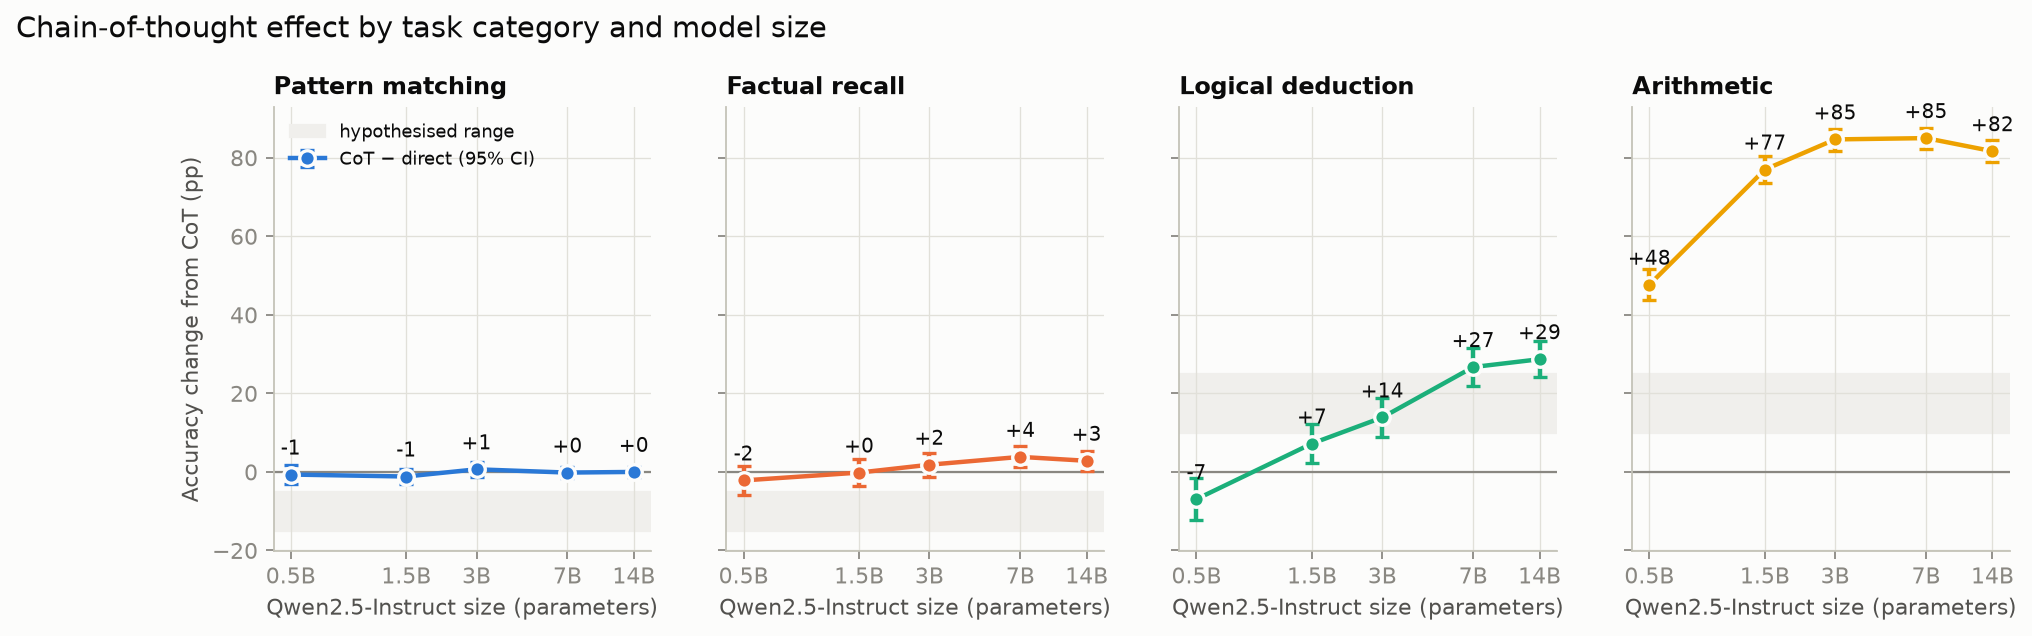
\includegraphics[width=0.98\linewidth]{figures/delta_by_category_scale.png}
    \caption{\CoT effect (\CoT minus direct accuracy, in points) by category and model size, with 95\% bootstrap intervals. Grey bands mark the hypothesised ranges. Pattern matching and factual recall stay near zero and never enter their band; logical deduction rises through its band with size; arithmetic sits far above its band.}
    \label{fig:delta}
\end{figure}

\subsection{Large gains on arithmetic, size-dependent gains on logic (H2)}
\label{sec:h2}

The direction of H2 holds from 1.5B up, but the magnitudes do not match.
Arithmetic gains are 2 to 8 times larger than the hypothesised 10--25 points.
This follows from the strict baseline: with the answer prefilled, models cannot show any working, and \direct accuracy on \synth is 0.0--0.3\% at every size (\tabref{tab:task}, \figref{fig:acc}).
Logical deduction is in range only at 3B ($+13.9$).
It is negative at 0.5B, below the range at 1.5B, and above it at 7B and 14B.

\proofwriter shows the contrast most clearly.
\direct accuracy stays near chance (29.7--39.7\%) at every size, while \CoT accuracy climbs from 24.7\% to 74.7\%.

\begin{table}[t]
    \centering
    \caption{Task-level accuracy (\%): direct $\rightarrow$ \CoT, with $\Delta$ in parentheses. Holm-significant $\Delta$ ($\alpha=0.05$, 40 tests) in {\bf bold}. No task shows a significant \CoT penalty at any size.}
    \label{tab:task}
    \resizebox{\textwidth}{!}{%
    \begin{tabular}{@{}lccccc@{}}
        \toprule
        \textbf{Task} & \textbf{0.5B} & \textbf{1.5B} & \textbf{3B} & \textbf{7B} & \textbf{14B} \\
        \midrule
        \agnews      & 83.0 $\rightarrow$ 84.3 ($+1.3$) & 83.3 $\rightarrow$ 79.7 ($-3.7$) & 81.3 $\rightarrow$ 83.3 ($+2.0$) & 88.3 $\rightarrow$ 87.3 ($-1.0$) & 86.7 $\rightarrow$ 87.3 ($+0.7$) \\
        \sst         & 87.7 $\rightarrow$ 85.0 ($-2.7$) & 92.0 $\rightarrow$ 93.3 ($+1.3$) & 93.3 $\rightarrow$ 92.7 ($-0.7$) & 93.7 $\rightarrow$ 94.3 ($+0.7$) & 95.7 $\rightarrow$ 95.0 ($-0.7$) \\
        \midrule
        \triviaqa    & 18.7 $\rightarrow$ 20.3 ($+1.7$) & 40.0 $\rightarrow$ 42.7 ($+2.7$) & 47.3 $\rightarrow$ 48.7 ($+1.3$) & 55.0 $\rightarrow$ 62.0 ($+7.0$) & 66.0 $\rightarrow$ 70.0 ($+4.0$) \\
        \mmlu        & 48.7 $\rightarrow$ 42.7 ($-6.0$) & 69.7 $\rightarrow$ 66.7 ($-3.0$) & 75.0 $\rightarrow$ 77.3 ($+2.3$) & 83.7 $\rightarrow$ 84.3 ($+0.7$) & 86.3 $\rightarrow$ 88.0 ($+1.7$) \\
        \midrule
        \bbh         & 24.0 $\rightarrow$ 18.8 ($-5.2$) & 26.4 $\rightarrow$ 33.2 ($+6.8$) & 43.6 $\rightarrow$ 50.0 ($+6.4$) & 54.4 $\rightarrow$ 74.8 ($\mathbf{+20.4}$) & 64.4 $\rightarrow$ 86.8 ($\mathbf{+22.4}$) \\
        \proofwriter & 33.3 $\rightarrow$ 24.7 ($-8.7$) & 35.7 $\rightarrow$ 43.3 ($+7.7$) & 29.7 $\rightarrow$ 51.0 ($\mathbf{+21.3}$) & 31.3 $\rightarrow$ 64.3 ($\mathbf{+33.0}$) & 39.7 $\rightarrow$ 74.7 ($\mathbf{+35.0}$) \\
        \midrule
        \gsm         & 4.3 $\rightarrow$ 37.3 ($\mathbf{+33.0}$) & 7.0 $\rightarrow$ 77.7 ($\mathbf{+70.7}$) & 14.0 $\rightarrow$ 89.0 ($\mathbf{+75.0}$) & 21.7 $\rightarrow$ 94.7 ($\mathbf{+73.0}$) & 32.0 $\rightarrow$ 97.3 ($\mathbf{+65.3}$) \\
        \synth       & 0.0 $\rightarrow$ 62.3 ($\mathbf{+62.3}$) & 0.0 $\rightarrow$ 83.3 ($\mathbf{+83.3}$) & 0.0 $\rightarrow$ 94.3 ($\mathbf{+94.3}$) & 0.0 $\rightarrow$ 97.0 ($\mathbf{+97.0}$) & 0.3 $\rightarrow$ 98.3 ($\mathbf{+98.0}$) \\
        \bottomrule
    \end{tabular}
    }
\end{table}

Four task-level cells have uncorrected $p < 0.05$ but do not survive correction: \proofwriter at 0.5B ($-8.7$, $p = 0.049$), \agnews at 1.5B ($-3.7$, $p = 0.027$), \proofwriter at 1.5B ($+7.7$, $p = 0.038$) and \triviaqa at 7B ($+7.0$, $p = 0.0025$, Holm $p = 0.061$).

\begin{figure}[t]
    \centering
    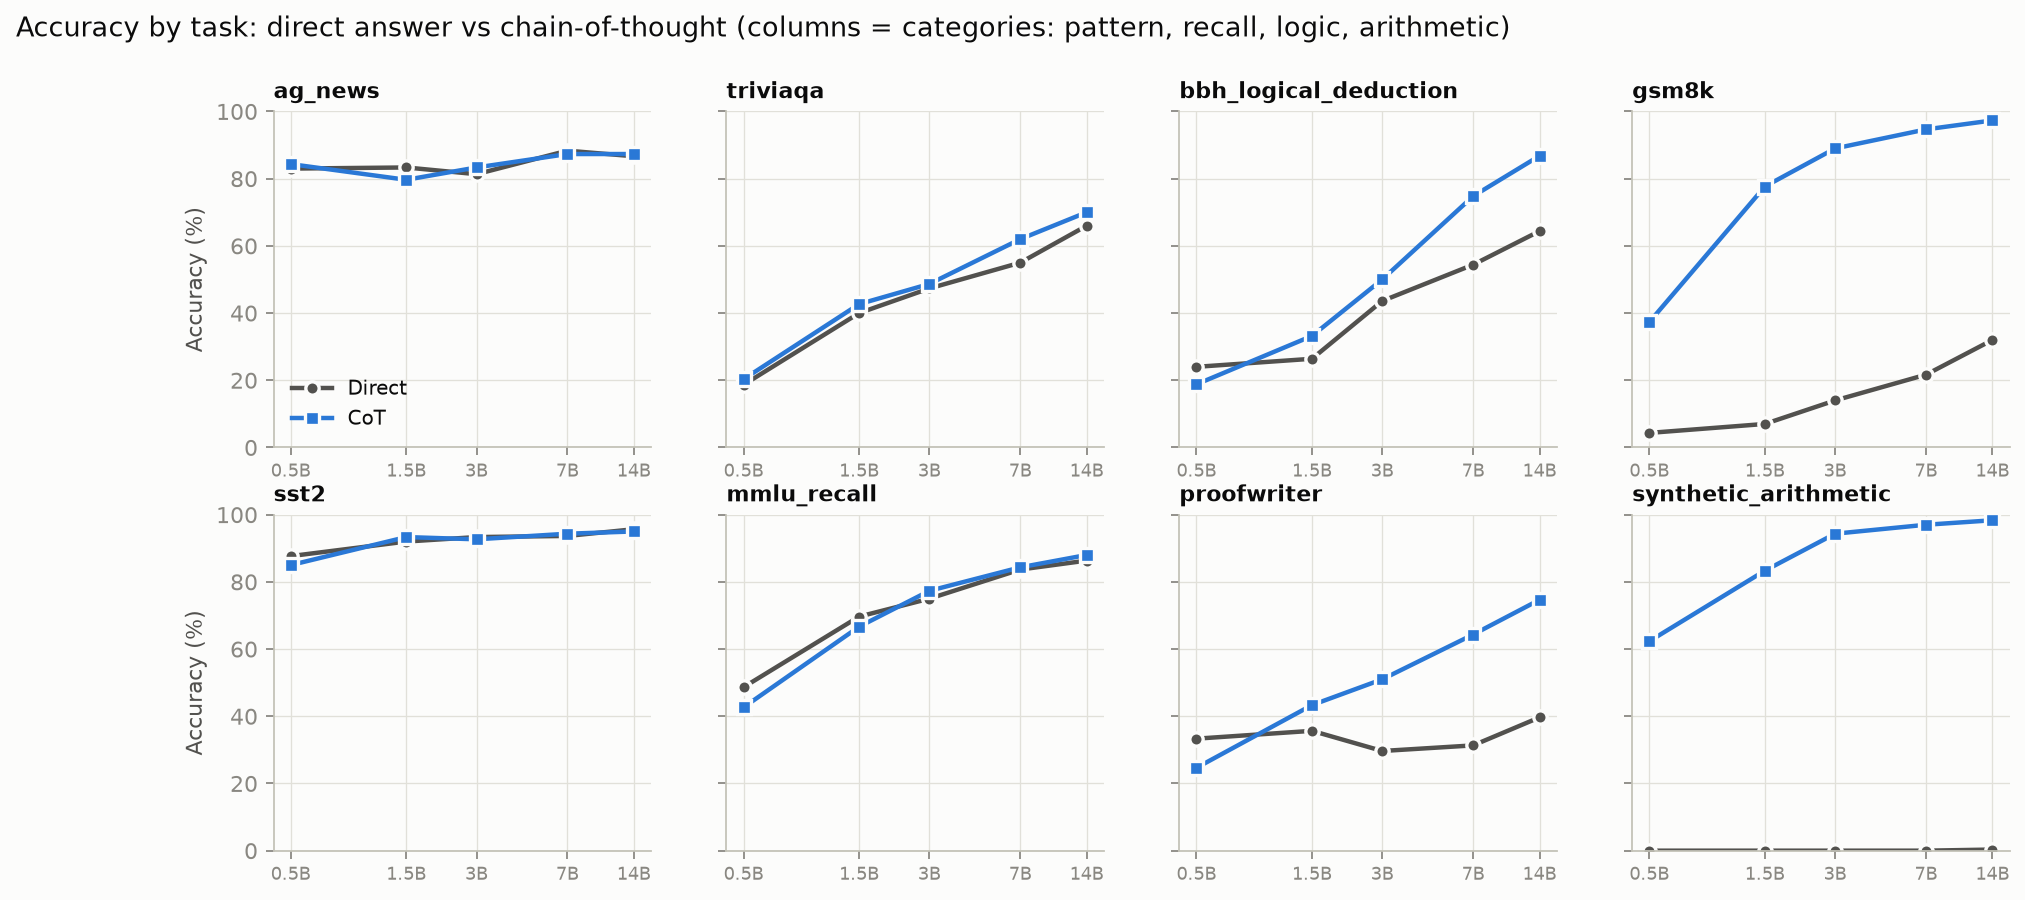
\includegraphics[width=0.98\linewidth]{figures/accuracy_by_task.png}
    \caption{Accuracy by task for direct answering and \CoT. Columns are categories (pattern matching, factual recall, logical deduction, arithmetic). The two conditions overlap on classification and recall; they separate with size on logic; on arithmetic the direct condition is near zero throughout.}
    \label{fig:acc}
\end{figure}

\subsection{The benefit of \CoT grows with scale (H3)}
\label{sec:h3}

H3 predicts that fewer categories benefit as models grow. We find the opposite (\tabref{tab:scale}).
\CoT significantly helps 2 of 8 tasks at 0.5B and 1.5B, 3 at 3B, and 4 at 7B and 14B.
No slope of $\Delta$ on $\log_2$(parameters) is negative.
The slope is $+7.6$ points per doubling for logical deduction and $+1.2$ for factual recall, and it is indistinguishable from zero for pattern matching.

The arithmetic slope ($+6.7$) needs a caveat: it comes almost entirely from the step from 0.5B to 1.5B.
From 3B up the arithmetic $\Delta$ is flat to slightly falling ($+84.7$, $+85.0$, $+81.7$).
On \gsm, $\Delta$ peaks at 3B ($+75.0$) and falls to $+65.3$ at 14B, because \direct accuracy keeps rising (14.0\% to 32.0\%) while \CoT accuracy approaches its ceiling (89.0\% to 97.3\%).

\begin{table}[t]
    \centering
    \caption{Scale trend. \figleft{} Number of tasks and categories with a Holm-significant \CoT effect at each size. \figright{} Slope of $\Delta$ per doubling of parameters, with 95\% bootstrap intervals.}
    \label{tab:scale}
    \footnotesize
    \begin{tabular}{@{}lccccc@{}}
        \toprule
        & \textbf{0.5B} & \textbf{1.5B} & \textbf{3B} & \textbf{7B} & \textbf{14B} \\
        \midrule
        Tasks helped (of 8) & 2 & 2 & 3 & 4 & 4 \\
        Tasks hurt (of 8) & 0 & 0 & 0 & 0 & 0 \\
        Categories helped (of 4) & 1 & 1 & 2 & 2 & 2 \\
        \bottomrule
    \end{tabular}
    \hfill
    \begin{tabular}{@{}lc@{}}
        \toprule
        \textbf{Category} & \textbf{Slope} \\
        \midrule
        Pattern matching & $+0.2$ {\scriptsize $[-0.3, +0.7]$} \\
        Factual recall & $+1.2$ {\scriptsize $[+0.3, +2.0]$} \\
        Logical deduction & $+7.6$ {\scriptsize $[+6.3, +8.9]$} \\
        Arithmetic & $+6.7$ {\scriptsize $[+5.7, +7.6]$} \\
        \bottomrule
    \end{tabular}
\end{table}

\subsection{Harm and fix rates}
\label{sec:harmfix}

A $\Delta$ near zero can hide offsetting changes, so we look at the two directions separately (\tabref{tab:harmfix}, \figref{fig:harmfix}).
Harm rates fall with size in every category: from 6.1\% to 1.3\% for pattern matching, 36.1\% to 5.0\% for factual recall, and 88.8\% to 9.6\% for logical deduction.
Fix rates rise with size in every category except pattern matching, where they fall from 30.7\% to 13.2\%.

Two cautions apply.
The arithmetic harm rates rest on very few items, because few arithmetic items are right in the direct condition (8 harmed items at 0.5B and 0--2 at other sizes).
And part of every harm and fix rate is run-to-run churn rather than an effect of \CoT (\secref{sec:limitations}), so $\Delta$ is the safer number.

\begin{table}[t]
    \centering
    \caption{Harm rate $P(\text{\CoT wrong} \mid \text{direct right})$ and fix rate $P(\text{\CoT right} \mid \text{direct wrong})$, in \%. Arithmetic harm rates rest on at most 8 harmed items per cell.}
    \label{tab:harmfix}
    \small
    \begin{tabular}{@{}lcccccccccc@{}}
        \toprule
        & \multicolumn{5}{c}{\textbf{Harm rate}} & \multicolumn{5}{c}{\textbf{Fix rate}} \\
        \cmidrule(lr){2-6} \cmidrule(lr){7-11}
        \textbf{Category} & 0.5B & 1.5B & 3B & 7B & 14B & 0.5B & 1.5B & 3B & 7B & 14B \\
        \midrule
        Pattern matching  & 6.1 & 4.4 & 2.7 & 1.6 & 1.3 & 30.7 & 21.6 & 23.7 & 14.8 & 13.2 \\
        Factual recall    & 36.1 & 17.0 & 10.6 & 5.5 & 5.0 & 15.1 & 20.3 & 21.5 & 25.0 & 28.0 \\
        Logical deduction & 88.8 & 45.1 & 35.9 & 18.7 & 9.6 & 26.4 & 31.3 & 42.9 & 60.3 & 69.6 \\
        Arithmetic        & 61.5 & 9.5 & 0.0 & 3.1 & 1.0 & 50.1 & 80.1 & 91.0 & 95.7 & 97.6 \\
        \bottomrule
    \end{tabular}
\end{table}

\begin{figure}[t]
    \centering
    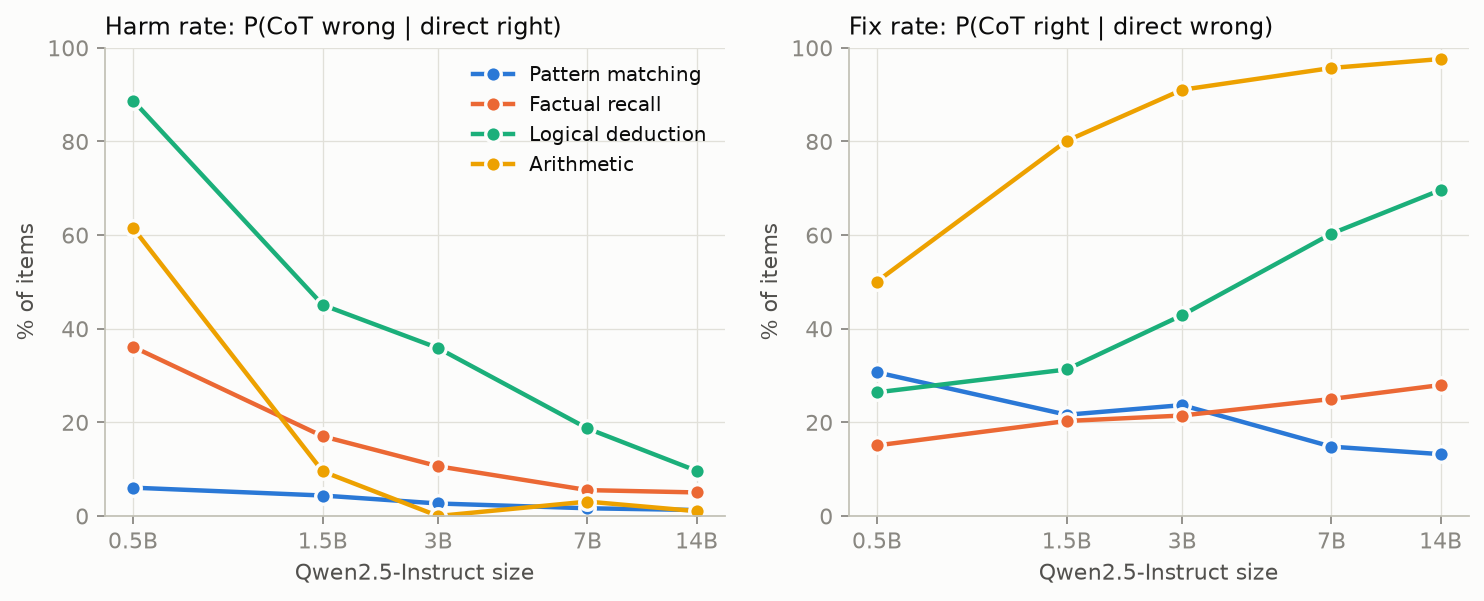
\includegraphics[width=0.8\linewidth]{figures/harm_fix_rates.png}
    \caption{Harm rates \figleft{} and fix rates \figright{} by category and model size. Harm rates fall with size in all four categories. Fix rates rise with size except for pattern matching.}
    \label{fig:harmfix}
\end{figure}

\subsection{Output diagnostics and token cost}
\label{sec:diag}

\para{Token cost.}
Mean output length is 3.1--3.3 tokens per item for \direct and 222--271 for \CoT, a ratio of 71$\times$ to 87$\times$ depending on the model.

\para{Well-formedness.}
\CoT responses carry an explicit answer marker and finish within budget in at least 95\% of cases for every model-task pair, with two exceptions on the smallest models.
On \synth the 0.5B model omits the marker in 24\% of responses; it ends with a boxed number, which the fallback parser reads.
On \proofwriter the small models often run out of budget: 44.0\% of \CoT responses hit the 1,024-token limit at 0.5B, 10.7\% at 1.5B, 5.0\% at 3B, 0.3\% at 7B and none at 14B.

\para{Where does the 0.5B loss on logic come from?}
The 0.5B model has 142 logical-deduction items that are right under \direct and wrong under \CoT.
Of these, 48 are truncated runs in which the model restates rule after rule until the budget runs out, 1 has no answer marker, and 93 give a wrong final answer.
When we restrict to items whose \CoT response is well-formed, logical deduction at 0.5B moves from $-6.9$ to $+3.7$ points ($n = 407$ of 550, interval $[-3.8, +11.1]$).
All other cells move by less than 2 points.
This subset is selected on the outcome of the \CoT run, so it shows where the loss comes from; it is not an unbiased estimate of what \CoT would do with a larger budget.

\subsection{Prompt robustness}
\label{sec:robust}

We repeat the comparison with the paraphrased instruction \cottwo on the first 100 items of each task (\tabref{tab:robust} in the appendix).
Across the 19 available model-by-category cells, the two wordings' effects correlate at 0.996.
Signs agree in 16 of 19 cells, and in the three disagreements both effects are within 4 points of zero.

This check has three weaknesses that we state plainly.
First, it is incomplete for 14B: out-of-memory errors on shared GPUs repeatedly killed that run, which finished 544 of 800 items and no logical-deduction items.
Second, with \cottwo, pattern matching shows small negative effects whose uncorrected intervals exclude zero for three models (0.5B: $-2.5$ $[-5.0, -0.5]$; 1.5B: $-2.5$ $[-5.0, -0.5]$; 14B: $-2.3$ $[-4.7, -0.5]$) and a positive one for 3B ($+3.5$ $[+0.5, +7.0]$).
These are uncorrected, rest on 200 or fewer items, and are mixed in sign, so we read them as bounding any classification penalty at roughly 2--5 points and not as evidence for one.
Third, on this 100-item subset the 0.5B effect on logical deduction is positive under both wordings ($+3.0$ and $+3.5$, with a \cottwo interval of $[-5.0, +12.0]$), unlike the $-6.9$ on the full set.
The negative cell in \tabref{tab:category} is therefore not stable across subsets of items.
